\documentclass[a4paper]{article}
\usepackage[margin=1.2in]{geometry}
\usepackage{graphicx}
\usepackage{tikz}
\usepackage{pgfplots}
\usepackage{xcolor}
\usepackage{listings}
\definecolor{codegreen}{rgb}{0,0.6,0}
\definecolor{codegray}{rgb}{0.5,0.5,0.5}
\definecolor{codepurple}{rgb}{0.58,0,0.82}
\definecolor{backcolour}{rgb}{0.95,0.95,0.92}
\lstdefinestyle{mystyle}{
    backgroundcolor=\color{backcolour},
    commentstyle=\color{codegreen},
    keywordstyle=\color{magenta},
    numberstyle=\tiny\color{codegray},
    stringstyle=\color{codepurple},
    basicstyle=\ttfamily\footnotesize,
    breakatwhitespace=false,
    breaklines=true,
    captionpos=b,
    keepspaces=true,
    numbers=left,
    numbersep=5pt,
    showspaces=false,
    showstringspaces=false,
    showtabs=false,
    tabsize=2
}
\lstset{language=c,style=mystyle}
\usepackage{booktabs}

\title{PPE Project Report\\Team 6}
\author{Hannah Atmer \and Xiaoyue Chen}
\date{October 2021}

\begin{document}

\maketitle
\tableofcontents

% Your grade on your project will be a combination of how challenging
% optimizations you choose, how well you implement them, and how well
% you analyze the results.

\section{Hardware}
\subsection{CPU}
\begin{verbatim}
Architecture              x86_64
CPU(s)                    12
Model name                Intel(R) Core(TM) i7-8750H CPU
Thread(s) per core        2
Core(s) per socket        6
CPU max MHz               4100.0000
\end{verbatim}

\subsection{GPU}
\begin{verbatim}
Device Name               NVIDIA GeForce GTX 1060
PCIe Version              3.0.0
Max compute units         10
Max clock frequency       1733MHz
Cuda cores                1280
\end{verbatim}

\section{Setup}
We used the following setup to encode 5 frames at 4k resolution:
\lstinputlisting[linerange=23-26]{src/test_setup.h}

\section{Motivation}
Table~\ref{tab:vanilla_breakdown} shows that the programme runs
extremely slow. Figure~\ref{fig:vanilla_callgraph} shows that most of
the time is spent on executing the Motion Vector Search function.

\begin{table}[h]
  \centering
  \begin{tabular}{ll}
    \toprule
    Function & Time (ms) \\
    \midrule
    Convert to YCbCr & 7000 \\
    Low pass filter & 10000 \\
    Motion Vector Search & 800000 \\
    Compute Delta &                1000 \\
    Downsample &                   1000 \\
    Convert to frequency domain &  3000 \\
    Quantize &                     2000 \\
    Compute DC differences &       50 \\
    Zig-zag order &                900 \\
    Encode coefficients &          3000 \\
    \midrule
    Total & 80000 \\
    \bottomrule
  \end{tabular}
  \caption{Breakdown of the total execution time of the original
    program}
  \label{tab:vanilla_breakdown}
\end{table}

\begin{figure}[h]
  \centering 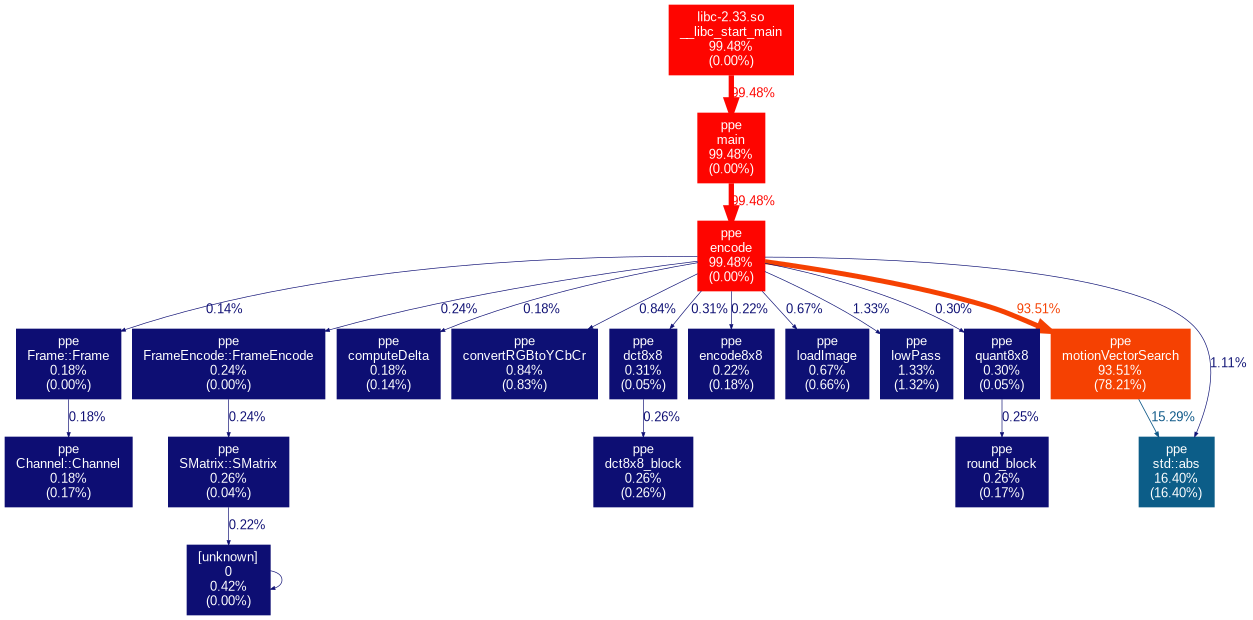
\includegraphics[height=6cm]{src/ppe-callgraph.png}
  \caption{Callgraph of the original program}
  \label{fig:vanilla_callgraph}
\end{figure}

After analysing both the table and the callgraph, we decided to
optimise the following functions because they took the longest to
execute: Motion Vector Search, Low-Pass Filter, Convert to YCbCr, and
Load Image.

\section{Optimisations}
\subsection{Motion Vector Search}
\subsubsection{Analysis}
Originally takes 93.51\% of runtime using 4K image sizes. This equals
around 100 seconds per frame. The slow execution is mainly due to
serve cache problems.

We found that the algorithm has the following properties:
\begin{itemize}
\item Task dependency exists only when finding the minimal SAD
\item Computational intensity \\
  \(> \frac{3_{op} \times (16 \times 16)_{InnerLoop} \times (33 \times 33)_{MiddleLoop} \times
    (254 \times 254)_{OuterLoop}}{(4096 \times 4096)_{FrameSize} \times 4_{byte}} =
  804\) OP/B \\
  is extremely high
\item There are \\
  \((33 \times 33)_{MiddleLoop} \times (254 \times 254)_{OuterLoop} = 65605\)
  parallelisable tasks
\end{itemize}

Given the properties of the algorithm, we decided to use the GPU to
speed up this comparison, and we used the map-reduce algorithm to
divide the work amongst GPU cores, collect the results, and reduce the
results to find the best match.

\subsubsection{Implementation}
We used OpenCL to implement the optimised function. When enqueuing the
kernel, the global dimension is \(4096 \times 4096\) (the entire image
size) and the local dimension is \(16 \times 16\) (the block size). Each
work-group is tasked to find the motion vector of a match block.

Another notable feature of this implementation is the good utilisation
of group-local memory. This improved the memory performance of GPU
significantly.

\lstinputlisting[caption=OpenCL implementation of Motion Vector
Search, firstline=15]{src/kernel.cl}

\subsubsection{Speedup}
We reduced the average execution time of the function from 500,000 ms
to 500 ms, which is a 1000x speedup. We achieved such impressive
speedup by utilising the group-local memory of our GPU very well.
Besides, distributing the tasks evenly to different threads also help
the performance.

\subsection{Low-Pass Filter}
\subsubsection{Analysis}
This algorithm has a lot of data dependencies. The results of the next
row depends on the results of the previous loop. Breaking the
dependencies would yield wrong results. Therefore, we need to be
careful when parallelising it using OpenMP.

We also noticed that we do not need to copy the entire frame at the
start of the function. Instead, we only need to copy the pixels on the
edges.

\subsubsection{Implementation}
We used OpenMP to optimise the function. We assign each thread a
number of columns to process because there is no data dependencies
across columns. We still use row major access in each thread to
utilise cache better. \lstinputlisting[caption=OpenMP optimisation of
Low-Pass Filter, linerange=113-175]{src/main.cpp}

\subsubsection{Speedup}
We reduced the average execution time of the function from 2,000 ms to
100 ms, which is a 20x speedup. The speedup is due to less copying,
better cache utilisation, as well as parallelism.

\subsection{Convert to YCbCr}
\subsubsection{Analysis}
The original function has cache utilisation problems. The algorithm is
trivially parallelisable since there is no data dependencies.

\subsubsection{Implementation}
We used OpenMP to optimised the function.
\lstinputlisting[caption=OpenMP optimisation of Convert to YCbCr,
linerange=80-97]{src/main.cpp}

\subsubsection{Speedup}
We reduced the average execution time of the function from 1,400 ms to
30 ms, which is a 46x speedup. The speedup is due to better cache
utilisation as well as parallelism.

\subsection{Other optimisations}
We complied our program using GCC with \verb|-msse4.1 -avx2 -O3|
flags. By checking the generated assembly, we found that GCC could
reliable issue AVX instructions as well as handle loop unrolling.
Optimisations from the compiler also improved the program's
performance.

\section{Results}
The results of our optimisation efforts could be summarised in
figure~\ref{fig:before_after_bar}. We achieved an overall speedup of
145x on the entire program. Most of the gain is from optimising the
Motion Vector Search (MVS) function which has seen a 1000x speedup.
\begin{figure}[h]
  \centering
  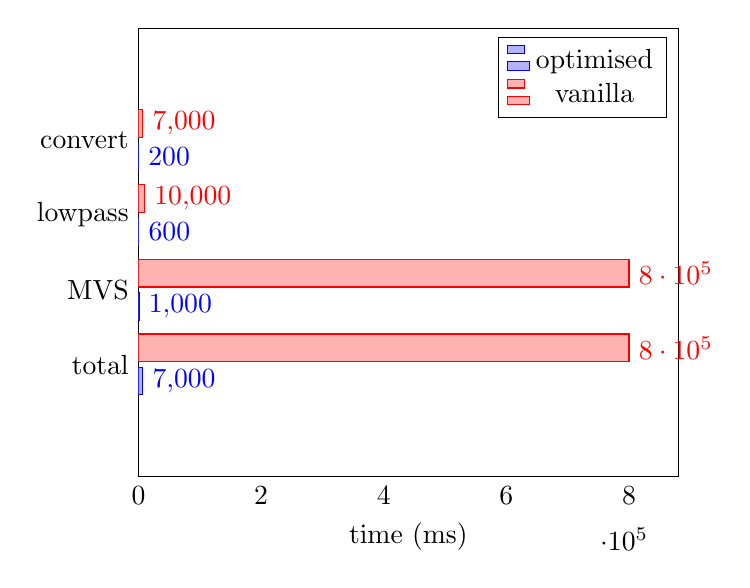
\begin{tikzpicture}
    \begin{axis}[xbar, xmin=0, enlarge y limits=0.5, tickwidth=0pt,
      xlabel={time (ms)}, ytick=data, symbolic y coords = {total, MVS,
        lowpass, convert}, nodes near coords ]
      \addplot coordinates {(200,convert) (600,lowpass) (1000,MVS)
        (7000,total)}; \addplot coordinates {(7000,convert)
        (10000,lowpass) (800000,MVS) (800000,total)};
      \legend{optimised, vanilla}
    \end{axis}
  \end{tikzpicture}
  \caption{Total execution time before and after optimisation}
  \label{fig:before_after_bar}
\end{figure}

\section{Discussion}
Most of the speedup is from optimising the Motion Vector Search (MVS)
function which has seen a 1000x speedup. It is also the most difficult
function for us to optimise. The difficulties come from in two
aspects:
\begin{enumerate}
\item The algorithm itself is complex and hard to understand
\item Using local memory introduces different index sets. We need to
  convert from group id of a thread to the index of the local arrays,
  as well as the index of the global array. The makes the kernel even
  more difficult to implement
\end{enumerate}

In spite of the difficulties, using OpenCL to do such low-level
optimisation is proven to be worth the effort, as the function is the
major bottleneck of the program.

\end{document}

%%% Local Variables:
%%% mode: latex
%%% TeX-master: t
%%% End:
